\documentclass[a4paper, 12pt]{article}

\def\languages{french, english}

%%%%%%%%%%%%%%%%%%% Libraries

\input{include/libraries/bibliography.tex}
\input{include/libraries/default.tex}
\input{include/libraries/figures.tex}
\input{include/libraries/informatics.tex}
\input{include/libraries/mathematics.tex}
\input{include/libraries/theorems.tex}
\input{include/libraries/units.tex}

%%%%%%%%%%%%%%%%%%% Titlepage

\def\logopath{resources/pdf/logo-uliege.pdf}
\def\toptitle{University of Liège}
\title{Frequency domain}
\def\subtitle{Linear control systems}
%\def\authorhead{Author}
\author{
    Bastien \textsc{Hoffmann} (20161283)\\
    Maxime \textsc{Meurisse} (20161278)\\
    Valentin \textsc{Vermeylen} (20162864)\\
}
%\def\rightauthorhead{}
%\def\rightauthor{}
\def\context{Master in Civil Engineering}
\date{Academic year 2019-2020}

%%%%%%%%%%%%%%%%%%% Options

\fancyhead[R]{}
\renewcommand{\thesubsection}{\arabic{subsection}}

%%%%%%%%%%%%%%%%%%% Document

\begin{document}
    % ----- Titlepage ----- %
    \input{include/titlepages/default.tex}
    
    % ----- Question 1 ----- %
    \subsection{Framework}
For this part of the work, we have decided to simplify our system and use 2 states instead of 4. The position and speed of the damper are therefore hidden in the force of the actuator, which is still the controllable input of our system.
\begin{figure}[H]
    \centering
    \includegraphics[width=0.7\textwidth]{resources/png/simplified-system.png}
    \caption{Simplified system of an active mass damper}
    \label{fig:simplified-system}
\end{figure}
The law that governs that system is the following : 
$$
m_{tot}\ddot{x} + c\dot{x} + kx = F_{wind} + F_{damper}
$$
where
\begin{itemize}
    \item $F_{damper} = m_{damper}a_{damper}$
    \item $m_{tot} = m_{building} + m_{damper}$
    \item $x$ is the position of the building relative to its rest position ($x = 0$)
\end{itemize}
Let's now define the input, output and states : 
\begin{itemize}
    \item $u_1 = F_{wind}$
    \item $u_2 = F_{damper}$
    \item $x_1 = x$
    \item $x_2 = \dot{x}$
    \item $y = x_1$ 
\end{itemize}
By doing so, our ABCD matrices are the following :
$$
A = \begin{pmatrix}
    0 & 1\\
    \dfrac{-k}{m_{tot}} & \dfrac{-c}{m_{tot}}\\
\end{pmatrix}
\quad
B = \begin{pmatrix}
    0 & 0\\
    \dfrac{1}{m_{tot}} & \dfrac{1}{m_{tot}}\\
\end{pmatrix}
$$
$$
C = \begin{pmatrix}
    1 & 0\\
\end{pmatrix}
\quad
D = \begin{pmatrix}
    0 & 0\\
\end{pmatrix}
$$

    
    % ----- Question 2 ----- %
    \subsection{Constraints and simulation specifications}
We have the following constraints : 
\begin{itemize}
    \item Acceleration of the mass damper between \num{0.3} and \num{0.6}$g$, as advised by Prof. Denoël.
    \item Power injected in the mass of below \SI{10}{\kilo\watt} so as to not have too much electrical consumption.
    \item Lateral movement of the top of the building not above \SI{1}{\meter}.
\end{itemize}
The two scenario we look at are the following : a turbulent wind of maximum \SI{810}{\kilo\newton}, that we represented as a sine function and a constant wind of the same intensity.\par
Here are the values of the different parameters we have chosen : 
\begin{table}[H]
    \centering
    \begin{tabular}{|l|c|c|}
        \hline
        {\bf Mass} & $m_{building} = \SI{1e7}{\kilogram}$ & $m_{damper} = \SI{3e3}{\kilogram}$\\ \hline
        {\bf Spring} & \multicolumn{2}{c|}{$k\approx\SI{4e8}{\newton\per\meter}$}\\ \hline
        {\bf Damper} & \multicolumn{2}{c|}{$c\approx\SI{1.3e6}{\newton\second\per\meter}$}\\ \hline
        {\bf Wind} & \multicolumn{2}{c|}{$F_{max} = \SI{810}{\kilo\newton}$}\\ \hline
    \end{tabular}
    \caption{Numerical values of the system}
    \label{tab:numerical-values}
\end{table}

% Choice of cross-over frequency
\subsubsection{Choice of cross-over frequency}
The frequency of our building is of about \SI{1}{\hertz}, as advised by Pr. Denoël, and the frequency of the sinusoidal wind we have decided to study is also of \SI{1}{\hertz}, so we have decided to use a cross-over frequency of \SI{5}{\hertz}. All frequencies above that, probably coming from noise and unwanted phenomena, will be attenuated, while the amplitudes of the frequencies below that, which correspond to the internals of our system, will be amplified.
$$
w_{co} = 2\pi f_{co} \approx \SI{30}{\radian\per\second}
$$

    
    % ----- Question 3 ----- %
    \subsection{Loop shaping}
The Bode plots of our open-loop system are given at figure \ref{fig:bode-ol}.
\begin{figure}[H]
    \centering
    \includegraphics[width=0.8\textwidth]{resources/png/bode-ol.png}
    \caption{Bode plots for 2D system.}
    \label{fig:bode-ol}
\end{figure}
As can be seen, every frequency is well attenuated, the high ones as well as the low ones.\par
At the cross-over frequency, the gain of the system is of about \SI{-215}{\deci\bel}. This is not what we want. We would like low frequencies to have a positive gain, high frequencies to have a negative one and the gain at the crossover frequency to be of \SI{0}{\deci\bel}.\par
Furthermore, we need a big enough phase margin at the crossover frequency to be resistant to the delays we will have in our system. In order to do that, we have decided to use a lead compensator as well as a gain. We will not need a low-pass filter as high frequencies will be well attenuated without it.

% Lead compensator
\subsubsection{Lead compensator}
Let's first start with the desired phase margin. Delays are discussed after, but we want to be able to respond at least to \SI{0.02}{\second} delays, which correspond to the \SI{50}{\hertz} of the actuator's piston \cite{iopscience_delay}.\par
We have decided to have a phase margin of \SI{70}{\degree}. In order to increase the phase margin at the crossover frequency, we have decided to use a lead compensator.\par
Its transfer function is given by : 
$$
G(s) = \dfrac{\frac{s}{w_z} + 1}{\frac{s}{w_p} +1}
$$
We now have to determine the values of the parameters $G_{LC}$, $w_z$ and $w_p$. For a given crossover frequency $\omega_{co}$ and a phase margin $\phi_m$, we can determine the two $w$ in the following way : 
$$
\left\{\begin{array}{l}
    {w_{z}=\tan (\alpha) w_{\mathrm{co}}} \\
    {w_{p}=\frac{w_{\mathrm{co}}}{\tan (\alpha)}}
\end{array}\right.
$$
with $\alpha = \frac{\pi}{4} - \frac{\phi_m}{2}$.\par
For our crossover frequency and our desired value of $\phi_m$, we get that : 
$$
w_z = \num{5.2898} \qquad w_p = \num{170.1385}
$$

% Gain
\subsubsection{Gain}
After that, we need to add a gain to our system in order to increase the amplitude gains for all frequencies and make it so that the amplitude is at \SI{0}{\deci\bel} at the crossover frequency. That is done by using a constant gain of \num{1.5178e9}. This does not affect the phase but increases the amplitudes of about \SI{183.6}{\deci\bel}, which positions our Bode plot to where we wanted it to be.

% Trade-offs
\subsubsection{Trade-offs}
The Bode and Nyquist plots of the controlled system are given at figures \ref{fig:bode-control} and \ref{fig:nyquist-control}. As can be seen, the desired results are obtained, and we have a phase margin of \SI{70}{\degree} on the Nyquist plot.
\begin{figure}[H]
    \centering
    \includegraphics[width=0.8\textwidth]{resources/png/bode-control.png}
    \caption{Bode plots of the controlled system}
    \label{fig:bode-control}
\end{figure}
\begin{figure}[H]
    \centering
    \includegraphics[width=0.8\textwidth]{resources/png/nyquist-control.png}
    \caption{Nyquist plot of the controlled system}
    \label{fig:nyquist-control}
\end{figure}
Concerning the impacts on the output signal and control input signal, they are in an acceptable range of values with the parameters we have chosen, as can be seen in figures \ref{fig:controllable-input} and \ref{fig:output}.
\begin{figure}[H]
    \centering
    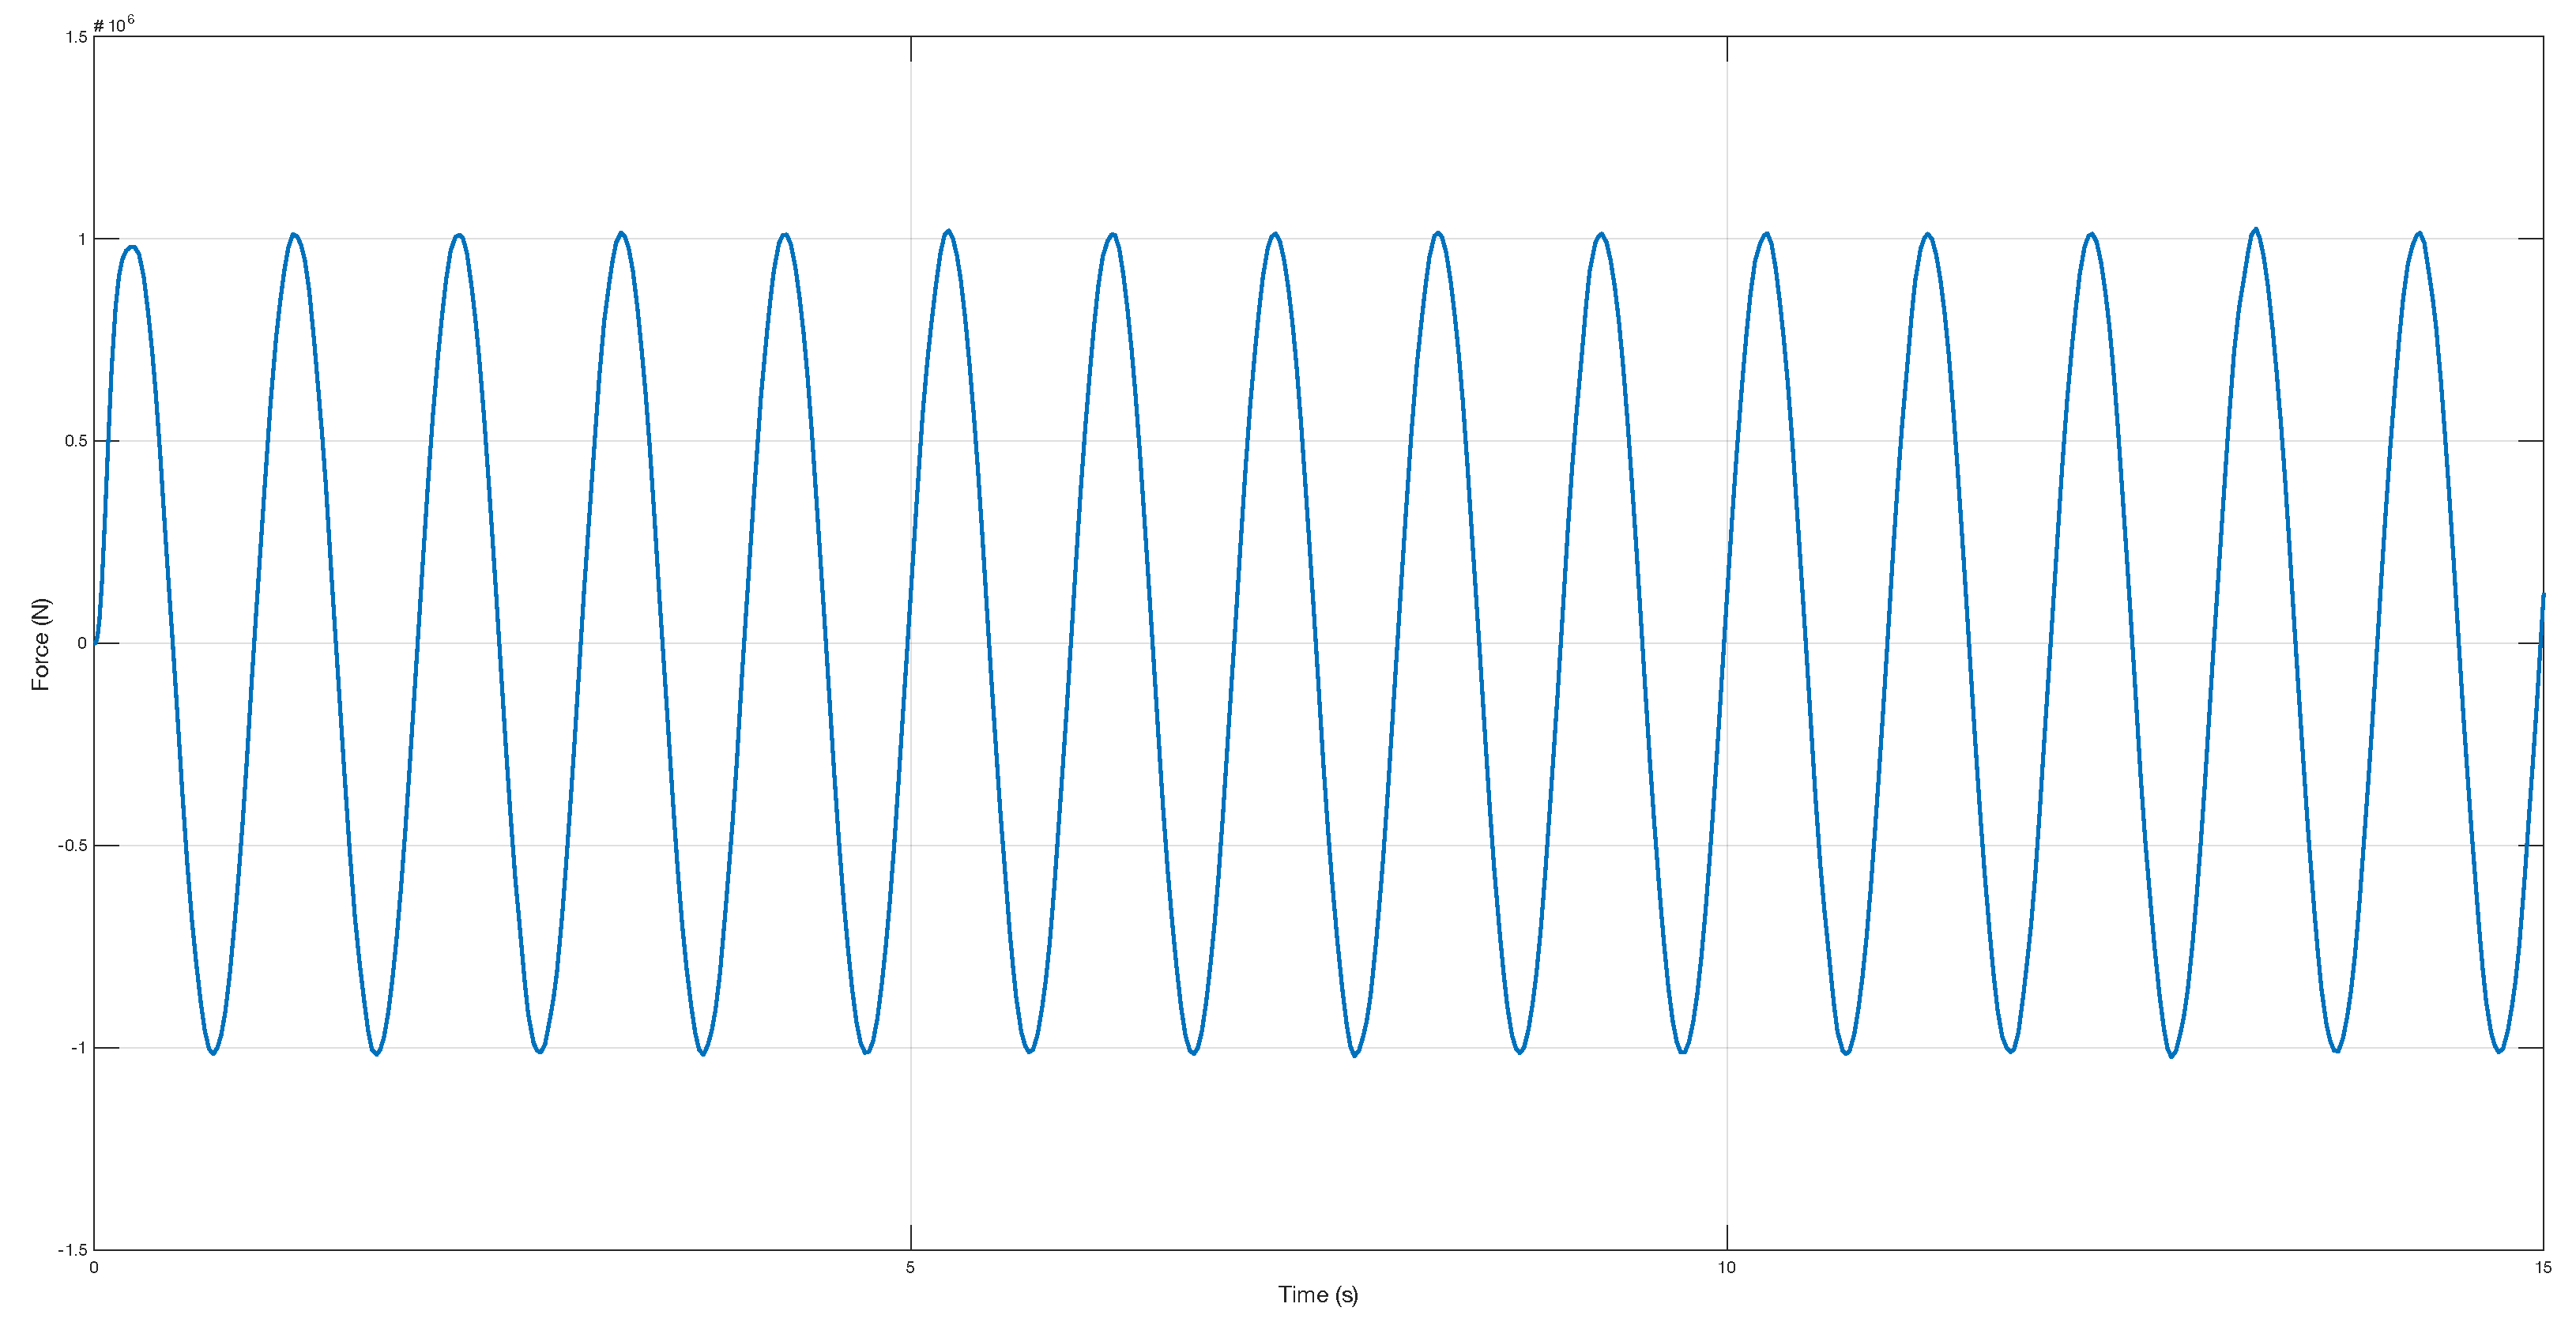
\includegraphics[width=0.8\textwidth]{resources/pdf/controllable-input.pdf}
    \caption{Plot of the controllable input of the controlled system}
    \label{fig:controllable-input}
\end{figure}
\begin{figure}[H]
    \centering
    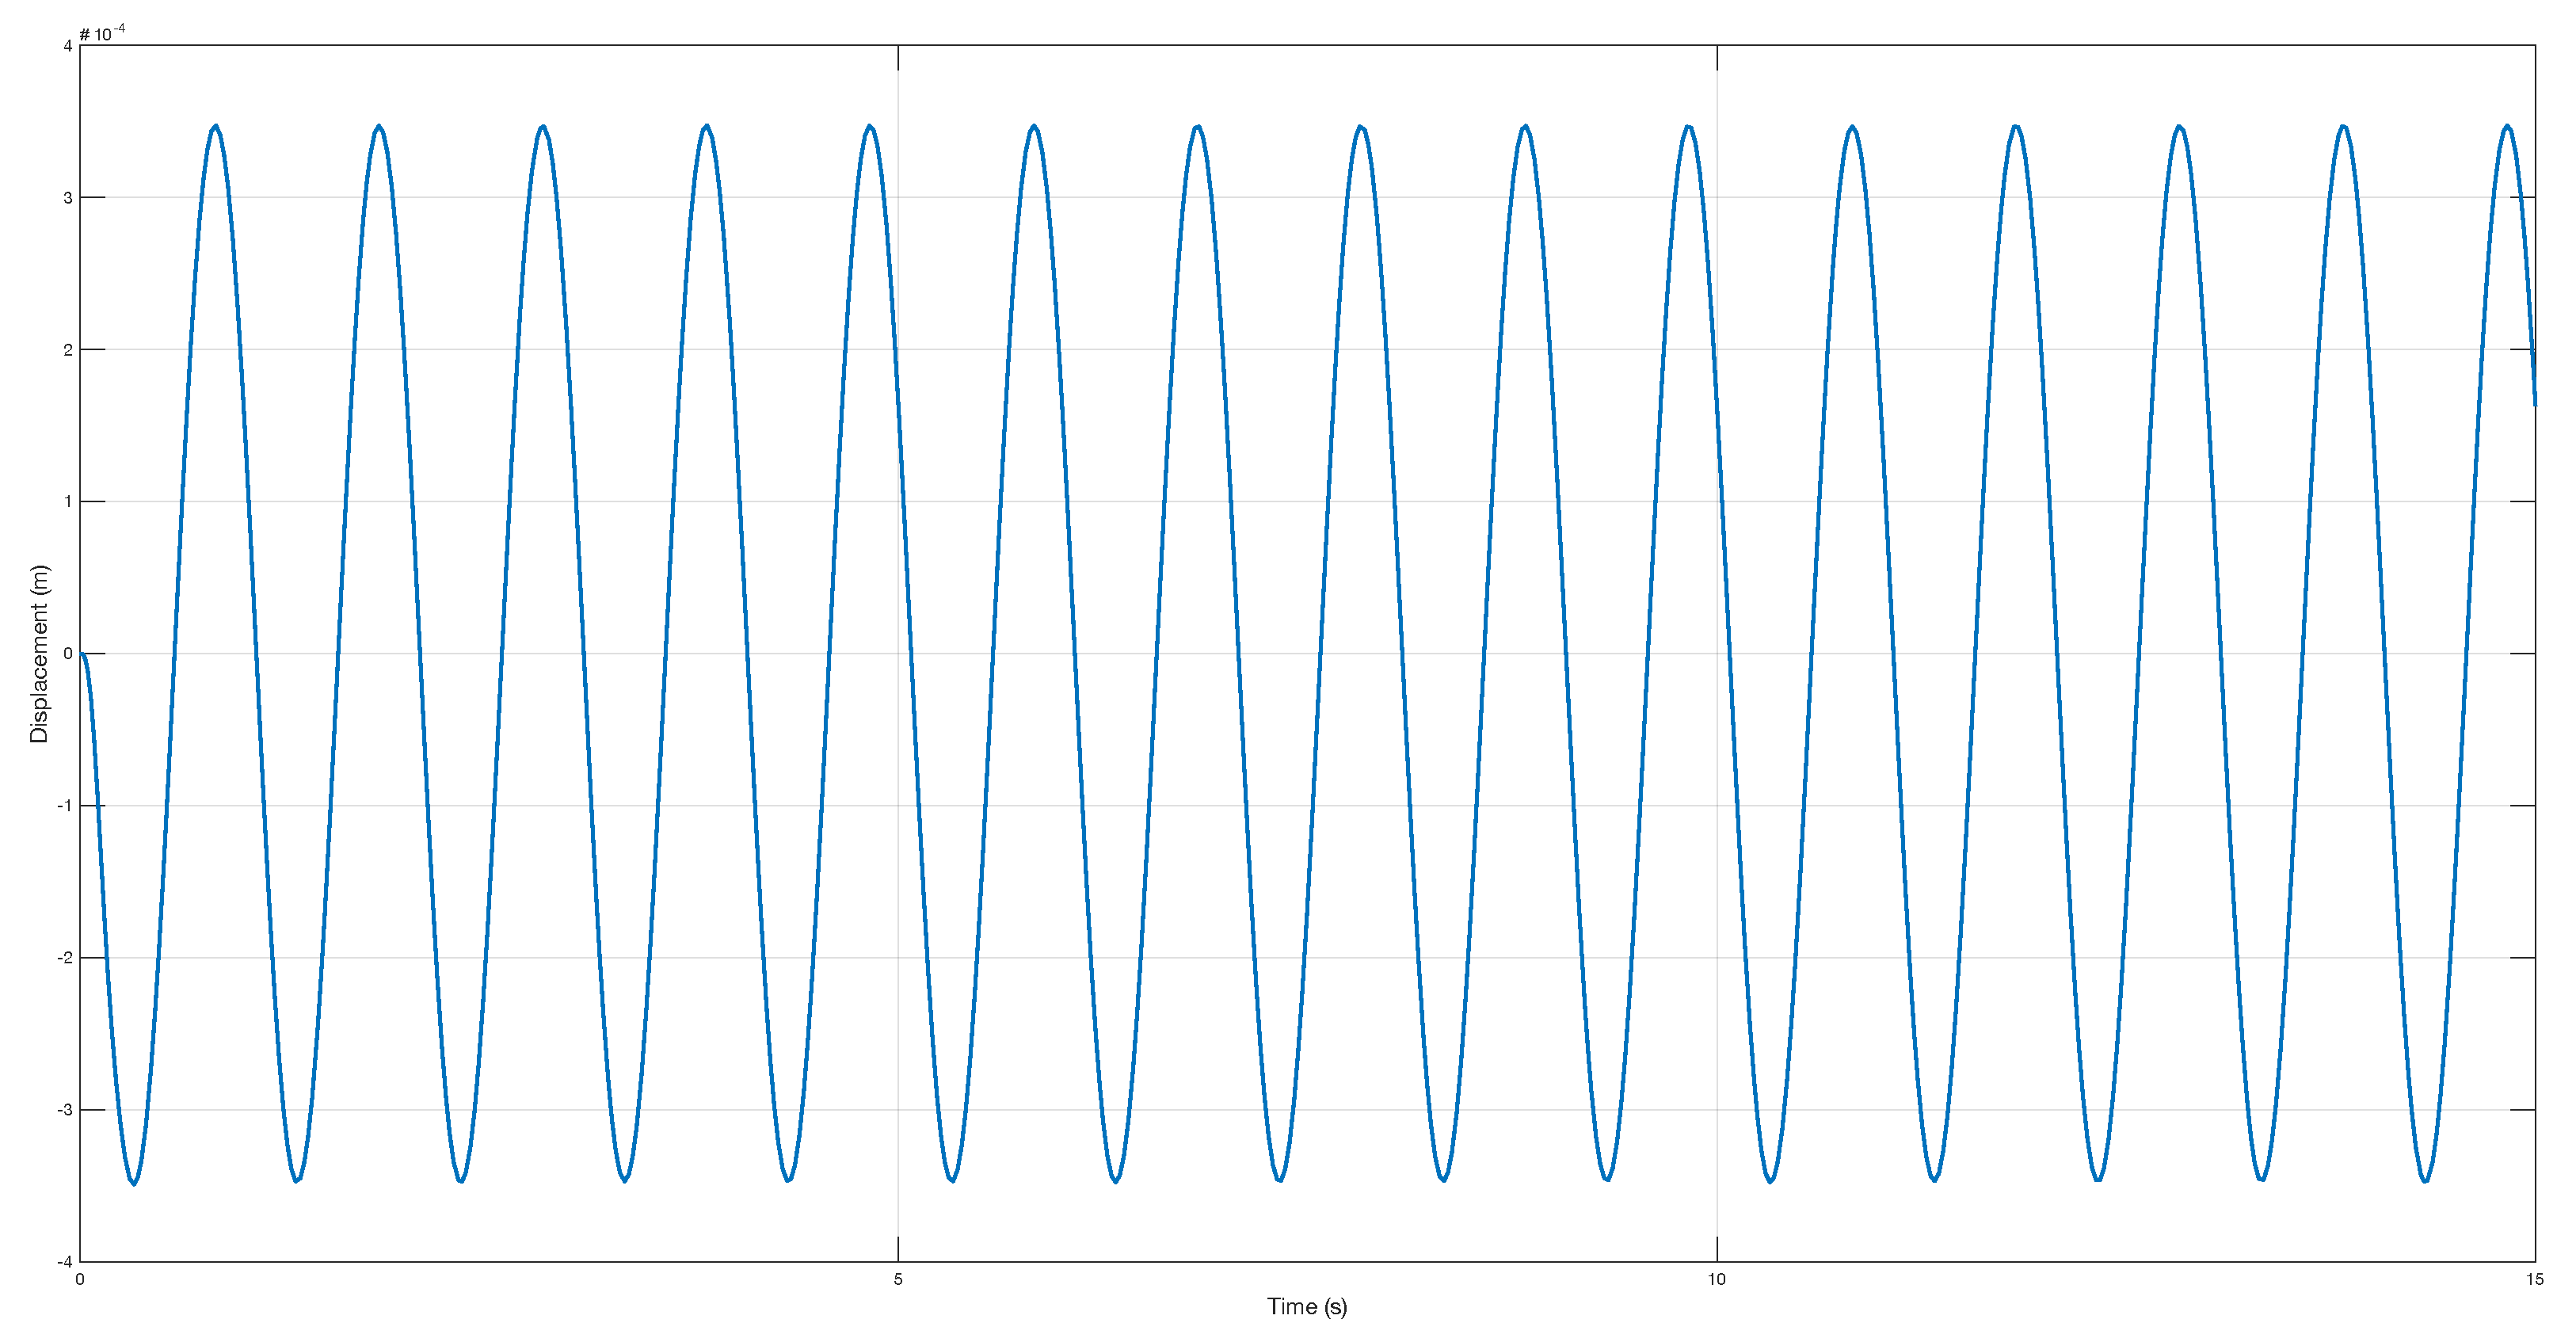
\includegraphics[width=0.8\textwidth]{resources/pdf/output.pdf}
    \caption{Plot of the output of the controlled system}
    \label{fig:output}
\end{figure}

    
    % ----- Question 4 ----- %
    \subsection{System simulations without controller}
To simulate the system (without control mechanism), we choose a series of numerical values, presented in table \ref{tab:numerical_values}\footnote{We would like to thank Professor Denoël for discussing these values with us.}.
\begin{table}[H]
    \centering
    \begin{tabular}{|l|c|c|}
        \hline
        {\bf Mass} & $m_1 = \SI{1e7}{\kilogram}$ & $m_2 = \SI{3e3}{\kilogram}$\\ \hline
        {\bf Spring} & $k_1 \approx \SI{4e8}{\newton/\meter}$ & $k_2 = \SI{e5}{\newton/\meter}$\\ \hline
        {\bf Damper} & $c_1 \approx \SI{1.3e6}{\newton\second/\meter}$ & $c_2 = \SI{e4}{\newton\second/\meter}$\\ \hline
        {\bf Wind} & \multicolumn{2}{c|}{$F_{max} = \SI{810000}{\newton}$}\\ \hline
    \end{tabular}
    \caption{Numerical values of the system}
    \label{tab:numerical_values}
\end{table}
For the strength of the wind, we considered 2 cases (in newton) :
\begin{align*}
    F_1 &= F_{max}\quad\forall t & \text{Constant wind force}\\
    F_1(t) &= F_{max}\sin(2\pi t) & \text{Sinusoidal wind force}
\end{align*}
The stiffness and viscosity values for the building were obtained using the formulas :
\begin{align*}
    k_1 &= (2\pi f)^2m_1\\
    c_1 &= 2m_1(2\pi f)0.01
\end{align*}
where $f = \SI{1}{\hertz}$ is the natural frequency associated with the mass of the building.\par
The maximum wind force, on the other hand, was approximated by
\begin{equation*}
    F_{max} = \frac{1}{2}\rho v^2A
\end{equation*}
with
\begin{itemize}
    \item $\rho \approx \SI{1.2}{\kilogram/\meter\cubed}$, the air density;
    \item $v = \SI{15}{\meter/\second}$, the wind speed;
    \item $A = 200\times 30 = \SI{6000}{\meter\squared}$, the area of one side of the building.
\end{itemize}
\subsubsection{Simulation results}
\begin{figure}[H]
    \centering
    \begin{subfigure}{0.495\textwidth}
        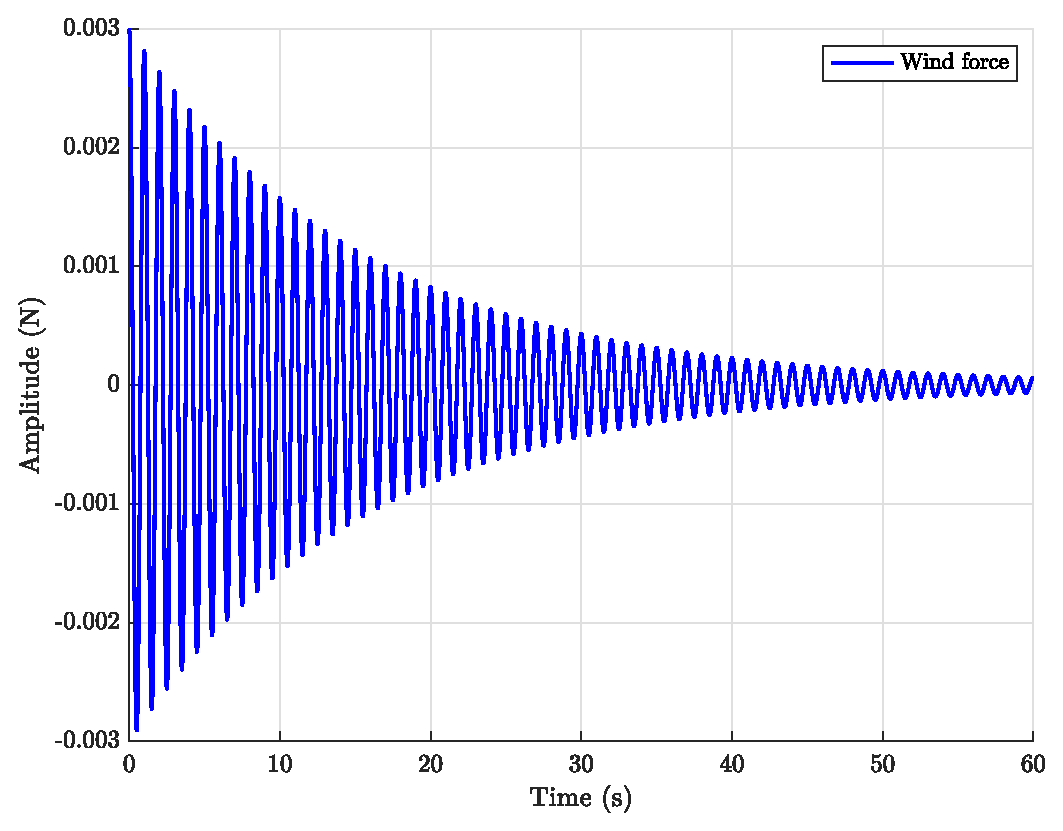
\includegraphics[width=\textwidth]{resources/eps/initial-condition.eps}
        \caption{Initial conditions}
        \label{fig:q4.initial}
    \end{subfigure}
    \begin{subfigure}{0.495\textwidth}
        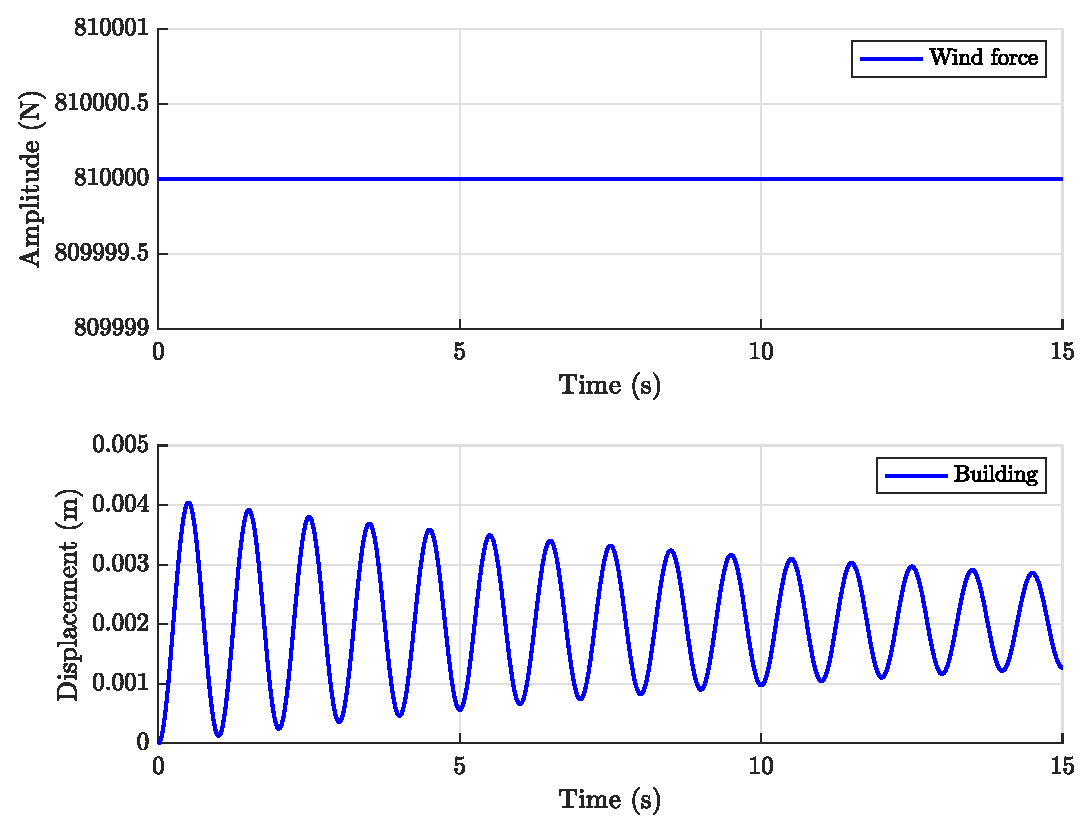
\includegraphics[width=\textwidth]{resources/eps/constant-wind.eps}
        \caption{Constant wind force}
        \label{fig:q4.constant}
    \end{subfigure}
    \begin{subfigure}{0.495\textwidth}
        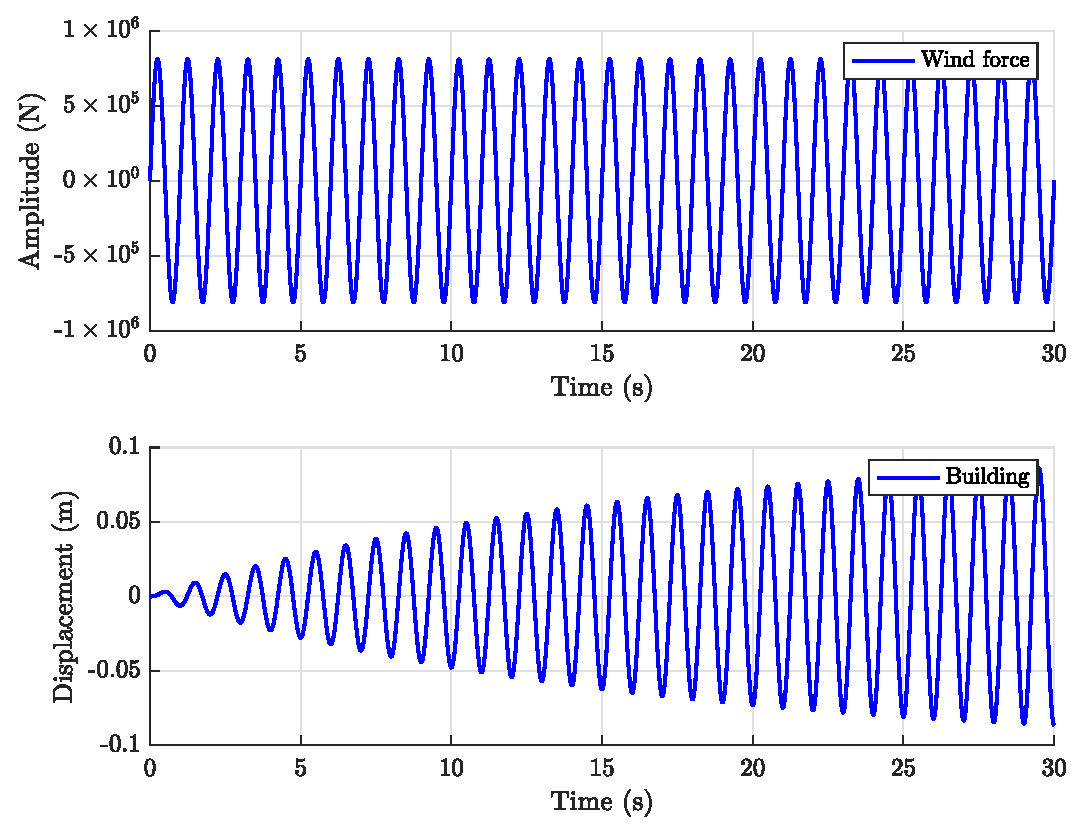
\includegraphics[width=\textwidth]{resources/eps/sinusoidal-wind.eps}
        \caption{Sinusoidal wind force}
    \end{subfigure}
    \begin{subfigure}{0.495\textwidth}
        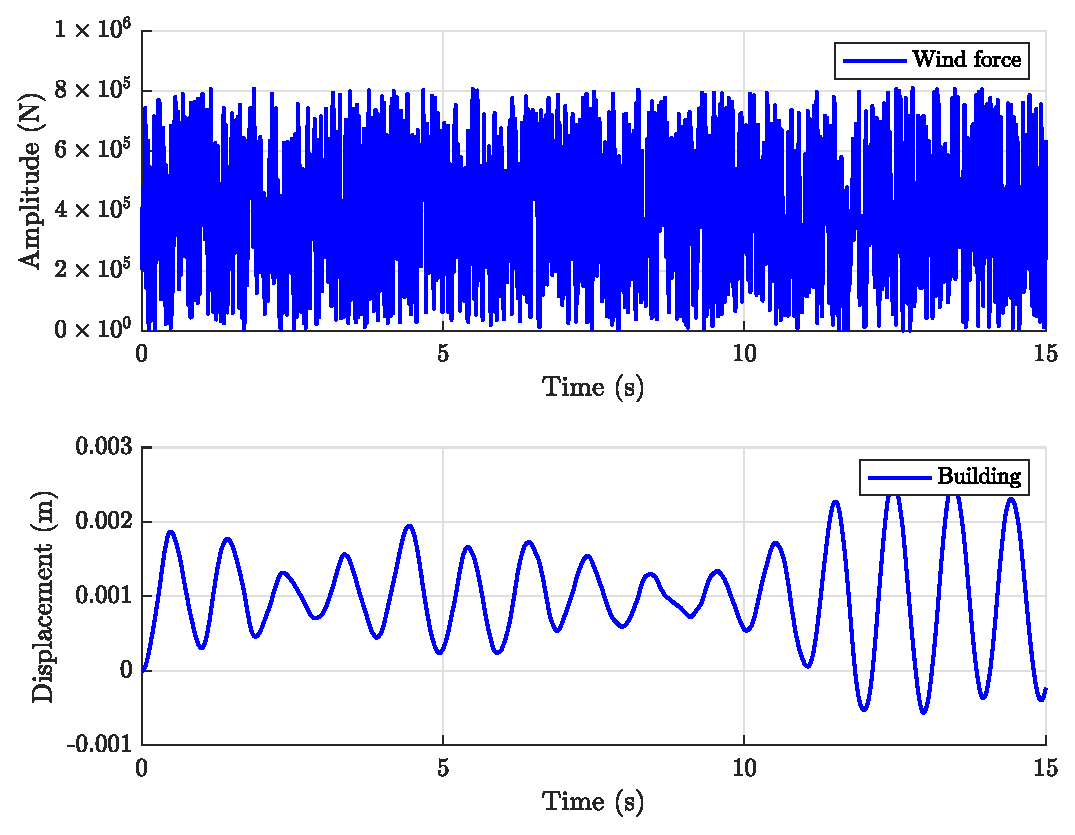
\includegraphics[width=\textwidth]{resources/eps/random-wind.eps}
        \caption{Random wind force}
    \end{subfigure}
    \noskipcaption{Simulation results}
\end{figure}
The first simulation (figure \ref{fig:q4.initial}) is a response of our system to initial conditions : the initial displacement of the building is defined at \SI{0.5}{\meter}. We observe that the building oscillates and tends to regain its reference position.\par
The other simulations are responses of our system to an input (the wind).\par
In the case of a constant force (figure \ref{fig:q4.constant}), the building oscillates at the beginning and then tends to stabilize (at a position different from its reference).\par
In cases of sinusoidal and random forces, the building oscillates and follows approximately the wind movement.

    
    % ----- Question 5 ----- %
    \subsection{Delays through the controller design}
to do

\end{document}
